 A basic event selection is made for selecting signal like events. The necessary event requirement are discussed in \Sec{sec:selection}. 

The analysis uses signal and background regions to constrain the huge \SM\ background compared to the expected signal. \Sec{sec:regions} discusses each region that is entering the analysis. On top of the use of background estimation from control regions, backgrounds that have  prompt leptons  contaminated by real leptons either
from decays of tau leptons or from hadronized mesons or baryons
(collectively commonly referred as ``non-prompt leptons") as well as by
hadrons or jets misidentified as leptons\footnote{These two classes
	of contamination will be referred to as not prompt-lepton (\NPL) samples.} are
evaluated with a data-driven method discussed in \Sec{sec:NPL}.
\section{Baseline event selection and filters}
Trigger and filters

Triggers used to select data events are given in Table \ref{tab:Trigger} and the trigger logic is based on \cite{CMSAN2016276}. The trigger paths are chosen based on on-line triggering objects with at least one muon (M), at least one electron (E), at least two muons (MM), at least two electrons (EE), at least one muon and an electron (ME), at least three muons (MMM), at least three electrons (EEE), at least two muons and one electron (MME), or at least two electrons and one muon (EEM). For the MC simulation a simple $or$ of all triggers is taken and the event is taken if it passes one of the trigger paths. For data however, double counting of the same event has to be taken into account and a procedure to avoid double counting has been put into place. It consists of vetoing in a given dataset the events that are already selected in another, as given in Table \ref{tab:triggerlogic}. 

\begin{table}[h]
	\centering
	\caption{HLT trigger paths used to select data events and the runs that they are applied to.}
	\begin{tabular}{c|c|c}
		\hline 
		Trigger path name & Applied on runs & Trigger type \\ 
		\hline 
		HLT\_Mu23\_TrkIsoVVL\_Ele8\_CaloIdL\_TrackIdL\_IsoVL\_v & All runs & ME \\ 
		%		\hline 
		HLT\_Mu23\_TrkIsoVVL\_Ele8\_CaloIdL\_TrackIdL\_IsoVL\_DZ\_v & All runs & ME \\ 
		%		\hline 
		HLT\_Mu8\_TrkIsoVVL\_Ele23\_CaloIdL\_TrackIdL\_IsoVL\_v & All runs & ME \\ 
		%		\hline 
		HLT\_Mu8\_TrkIsoVVL\_Ele23\_CaloIdL\_TrackIdL\_IsoVL\_DZ\_v & All runs & ME \\ 
		%		\hline 
		HLT\_DiMu9\_Ele9\_CaloIdL\_TrackIdL\_v & All runs & MME \\ 
		%		\hline 
		HLT\_Mu8\_DiEle12\_CaloIdL\_TrackIdL\_v & All runs & EEM \\ 
		\hline 
		HLT\_IsoMu24\_v & All runs & M \\ 
		%		\hline 
		HLT\_IsoTkMu24\_v & All runs & M \\ 
		\hline 
		HLT\_Ele32\_eta2p1\_WPTight\_Gsf\_v & All runs & E \\ 
		\hline 
		HLT\_Mu17\_TrkIsoVVL\_Mu8\_TrkIsoVVL\_v & All runs & MM \\ 
		%		\hline 
		HLT\_Mu17\_TrkIsoVVL\_TkMu8\_TrkIsoVVL\_v & All runs & MM \\ 
		%		\hline 
		HLT\_Mu17\_TrkIsoVVL\_Mu8\_TrkIsoVVL\_DZ\_v & All runs & MM \\ 
		%		\hline 
		HLT\_Mu17\_TrkIsoVVL\_TkMu8\_TrkIsoVVL\_DZ\_v & All runs & MM \\ 
		%		\hline 
		HLT\_TripleMu\_12\_10\_5\_v & All runs & MMM \\ 
		\hline 
		HLT\_Ele23\_Ele12\_CaloIdL\_TrackIdL\_IsoVL\_DZ\_v & All runs & EE \\ 
		HLT\_Ele16\_Ele12\_Ele8\_CaloIdL\_TrackIdL\_v & All runs & EEE \\ 
		\hline 
	\end{tabular} 
	\label{tab:Trigger}
\end{table}

\begin{table}[h]
	\centering
	\caption{Trigger logic used to select data events in order to avoid double counting}
	\begin{tabular}{c|c}
		\hline 
		Dataset & Trigger Logic \\ 
		\hline 
		/MuonEG/ & EM $\Arrowvert$ EEM $\Arrowvert$ MME \\ 
		\hline 
		/DoubleMu/ & (MM $\Arrowvert$ MMM) \&\& !( EM $\Arrowvert$ EEM $\Arrowvert$ MME)  \\ 
		\hline 
		/DoubleEG/ & (EE $\Arrowvert$ EEE) \&\& !(MM $\Arrowvert$ MMM) \&\& !( EM $\Arrowvert$ EEM $\Arrowvert$ MME) \\ 
		\hline 
		/SingleMuon/ & M \&\& !(EE $\Arrowvert$ EEE) \&\& !(MM $\Arrowvert$ MMM) \&\& !( EM $\Arrowvert$ EEM $\Arrowvert$ MME) \\ 
		\hline 
		/SingleElectron/ & E \&\& !M \&\& !(EE $\Arrowvert$ EEE) \&\& !(MM $\Arrowvert$ MMM) \&\& !( EM $\Arrowvert$ EEM $\Arrowvert$ MME)  \\ 
		\hline 
	\end{tabular} 
	\label{tab:triggerlogic}
\end{table}

\newpage
This trigger selection strategy is to allow the maximum statistics on the signal region since it does not  discard events from any dataset. The lowest \pt\ thresholds of the unprescaled three lepton triggers are \pt $>$16, 12, 6 \GeV\ for electrons, and \pt\ $>$12, 10, 5 \GeV\ for muons. For the dilepton triggers, these are   \pt\ $>$17, 12 \GeV for electrons and  \pt\ $>$17, 8 \GeV\ for muons. The single lepton triggers are used to complete the trigger efficiency for higher \pt.
Since the off-line \pt\ thresholds (given in Section \ref{sec:sel}) are much higher than the on-line trigger thresholds, a full trigger efficiency is guaranteed. The trigger efficiency estimation is described in Section \ref{sec:triggereff}.



The samples are pre-selected off-line to ensure that all reconstructed particles considered for the analysis are corresponding to a proton interaction and that signals from beam halo particles as well as detector noise is removed. For this reason, several filters are used \cite{MET,MUOtop}:

\begin{description}
	\item[Primary vertex] Only events with where the first primary vertex is a well reconstructed primary vertex are selected. The reconstructed primary vertex should have at least five degrees of freedom, the longitudinal distance from the beam spot is maximally 24 cm ($d_z < 24$ cm), and the transversal distance from the beam spot is maximally 2 cm ($d_{xy}<2$ cm ). (Applied on data and MC.)
	\item [Beam halo] The machine induced particles, via beam-gas / beam-pipe/... interactions, that are flying with the beam affect the physics analysis. Therefore, events containing such beam halo particles are removed from the selection with the CSC Beam Halo Filter. (Applied on data and MC.)
	\item [HBHE and HBHEiso noise] The HBHE is known to record sporadic anomalous signals (noise) at a fixed rate independent of the beam conditions. The events are cleaned for this noise. (Applied on data and MC.)
	\item 
	[ee badSC noise]  There are two supercrystal regions that give anomalous high energies and events suffering from this problem have to be removed. (Applied on data only.) 
	\item [ECAL TP] The ECAL dead cell trigger primitive filter is used to correct for channels where the primary data links were down during data taking. It also corrects for ECAL noisy crystals that were masked during the reconstruction of the event. (Applied on data and MC.)
	\item [badMuon] There is a reconstruction issue leading to high \pt\ muons at $\abs{\eta}>2.3$. This causes multi-\TeV\ range in MET for both MC and data. (Applied on data and MC.)
	\item[badCharged hadron] There is a reconstruction issue leading to high \pt\ muons at $\abs{\eta}>2.3$, when these muons are low quality, they are labelled as a hadron. This causes multi-\TeV/ range in MET for both MC and data. (Applied on data and MC.)
	\item[bad event muon]  The events containing at least one bad PF muon with a \pt\ above 20 \GeV\ that is flagged as bad are removed. (Applied on data and MC.)
	\item[bad clone muon] The events containing at least one PF muon with a \pt\ above 20 \GeV\ that is flagged as a duplicate are removed. (Applied on data and MC.)
\end{description}

% see https://indico.cern.ch/event/591506/contributions/2387636/attachments/1381281/2099935/2016_12_01_MET_Scanning_Report_PPD.pdf
% see https://indico.cern.ch/event/537458/contributions/2184619/attachments/1281045/1903148/met_scanner_report_may30.pdf
% see https://indico.cern.ch/event/534040/contributions/2178680/attachments/1280427/1901837/HCALnoise_JamboreeMeeting_27May2016.pdf
%see https://indico.cern.ch/event/518559/contributions/2132815/attachments/1264581/1871184/beamhalostatus.pdf
% see https://twiki.cern.ch/twiki/bin/viewauth/CMS/MissingETOptionalFiltersRun2


\subsection{Estimation of the trigger efficiency}
\label{sec:triggereff}
The trigger efficiency in data is estimated using a data sample collected using unprescaled MET triggers, following the approach of \cite{CMSAN2016276}. The events passing the trigger paths:
\begin{itemize}
	\item HLT\_PFHT300\_PFMET110\_v*, or
	\item HLT\_MET200\_v*, or 
	\item HLT\_PFMET300\_v*, or
	\item HLT\_PFMET120\_PFMHT120\_IDTight\_v*, or
	\item HLT\_PFMET170\_HBHECleaned\_v*
\end{itemize}
are being considered for the test data sample. These trigger paths are chosen to be completely uncorrelated with the lepton triggers given in Table \ref{tab:Trigger}. The studied simulation sample is the main background, \WZ+jets, with all corrections applied. For this study, the events passing a three lepton cut and at least one jet present, are being used. The corresponding efficiencies are then calculated as
\begin{equation}
\epsilon_{data} = \frac{\textnormal{Nb. of events passing lepton and MET triggers}}{\textnormal{Nb. of events passing MET triggers}}
\end{equation}
\begin{equation}
\epsilon_{MC} = \frac{\textnormal{Nb. of events passing lepton triggers}}{\textnormal{Nb. of total events}}
\end{equation}
The resulting efficiencies and scale factors can be found in Table \ref{tab:trigSF} and \ref{tab:trigSFe}, where the scale factors are defined as 
\begin{equation}
SF = \frac{\epsilon_{data}}{\epsilon_{MC}}.
\end{equation} 

\begin{table}[h]
	\centering
	\caption{Trigger scale factors for each channel, after three lepton + jets cut, in the Z mass window. by counting number of events.}
	\begin{tabular}{c|c|c|c|c}
		\hline 
		all & \mumumu & \eee & \eemu & \emumu \\ 
		\hline 
		1.0000 & 1.0000 & 0.9541 & 1.0006  & 1.0004\% \\ 
		\hline 
	\end{tabular} 
	\label{tab:trigSFe}
\end{table}

The trigger efficiencies are also measured in function of the \pt\ of the leptons. The resulting histograms can be found in Appendix \ref{app:trig}, the resulting scale factors in can be found in Figure \ref{image:FigurestriggerIntext}.
%\begin{figure}[tb]
%	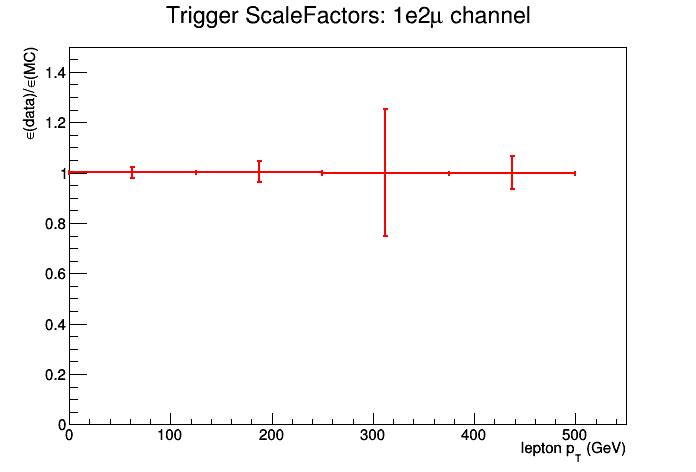
\includegraphics[width=0.48\textwidth]{Figures/trigger/Intext/SF_trigger_1e2muhistPt.png}
%	%		\label{image:SF_trigger_1e2muhistPt.png}
%	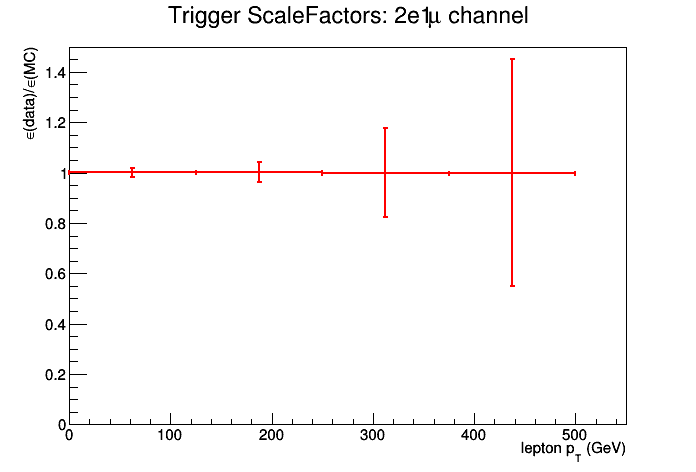
\includegraphics[width=0.48\textwidth]{Figures/trigger/Intext/SF_trigger_2e1muhistPt.png}
%	%		\label{image:SF_trigger_2e1muhistPt.png}
%	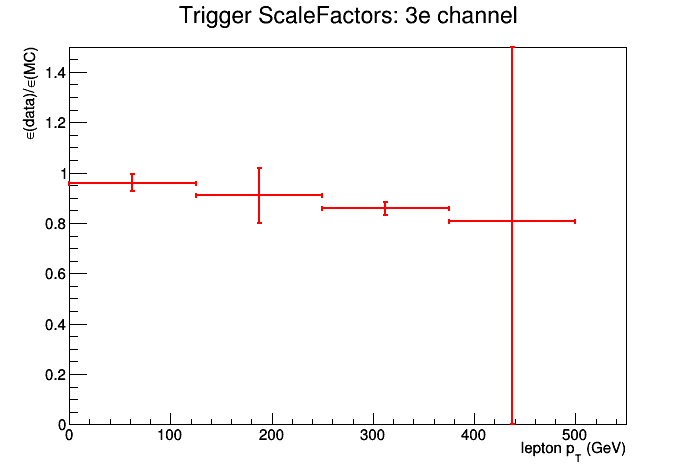
\includegraphics[width=0.48\textwidth]{Figures/trigger/Intext/SF_trigger_3ehistPt.png}
%	%		\label{image:SF_trigger_3ehistPt.png}
%	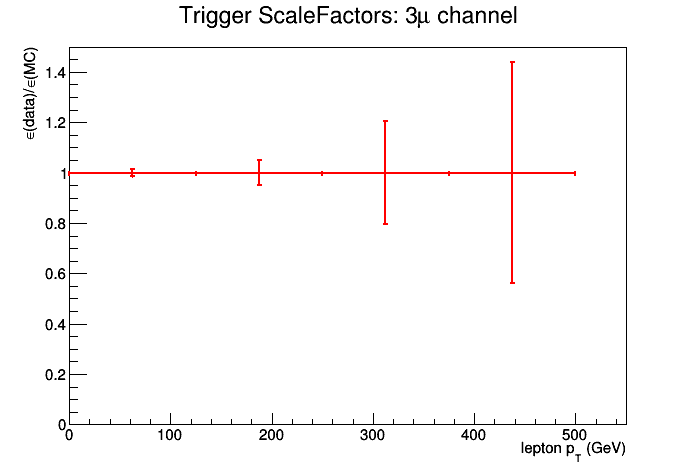
\includegraphics[width=0.48\textwidth]{Figures/trigger/Intext/SF_trigger_3muhistPt.png}
%	%		\label{image:SF_trigger_3muhistPt.png}
%	
%	\caption{The trigger scale factors measured as a function of lepton \pt, using the dataset collected by \Etmis\ triggers and \WZ\ simulation, after a 3 lepton and jets selection, in the Z mass window. All corrections to simulation are applied. Left, upper: 1e2$\mu$ channel. Right, upper: 2e1$\mu$ channel. Left, lower: 3e channel. Right, lower: 3$\mu$ channel}
%	\label{image:FigurestriggerIntext}
%\end{figure}
As can be seen from Appendix \ref{app:trig}, the trigger efficiencies are measured to be nearly 100\% for both simulation and data. The results are dominated by statistics and assigning a large uncertainty to the trigger efficiency based on the dataset collected by \Etmis\ triggers would be over conservative. A one percent uncertainty on the trigger selection for the \eemu\ and \mumumu\ final states, and 5\% for the \eee\ and \emumu\ final states, following the approach of \cite{Sirunyan:2017kkr}, while no scale factors will be applied on simulation as they are close to unity. Control plots are made in the dilepton region to validate all corrections applied to simulation and can be found in Appendix \ref{app:controldilep}.


\section{Event selection}
\label{sec:selection}
%met filter %http://cds.cern.ch/record/2205284/files/JME-16-004-pas.pdf
\section{Effect of the corrections in dilepton events}
\section{Signal and control regions}
The regions are defined as in Table \ref{tab:Regions} after a common selection of
\begin{itemize}
	\item exactly 3 leptons containing one opposite sign, same flavour pair,
	\item at least 1 jet and at the most 3 jets,
	\item the transverse mass of the \PW\ boson to be maximal 300 \GeV,
\end{itemize}
The cut on the transverse mass of the \PW\ boson is done to remove events that are passing the events cleaning although they shouldn't.
The transverse mass $\mtw$ is reconstructed using
\begin{equation}
\mtw = \sqrt{(\pt(l_{\W}) + \pt(\nu_{\W}) ) ^2 - (p_{\mathrm{x}}(l_{\W}) + p_{\mathrm{x}}(\nu_{\W}))^2  - (p_{\mathrm{y}}(l_{\W}) + p_{\mathrm{y}}(\nu_{\W}))^2    }
\end{equation}



Additional leptons are vetoed in order to reduce the contamination of backgrounds with four or more leptons in the final state, e.g. \ZZ, \ttZ, and \ttH. The most important backgrounds are the ones that contain three prompt leptons in the final state. These are mainly \WZ +jets, \ttZ and SM \tZq. For these backgrounds, the three lepton topology is identical to the \FCNC\ signal: two opposite sign leptons of the same flavour decaying from the \PZ\ boson, and a third additional, high \pt\ lepton coming from the \PW\ boson decay.

For the FCNC \tZ\ final state, one b jet coming from the SM top decay is expected. For the FCNC \tZq, an additional light jet is expected. In the \ttZ\ final state, two b jets are present in the final state. However, due to inefficiencies of the b-tagging algorithm, one of the two b jets may be identified as a light quark jet, giving the same final state as the FCNC \tZq\ final state. For the \WZ+jets final states, one of the b jets produced by gluon splitting can be b-tagged or light flavour jets coming from the \WZ+jets production can be mis-tagged as b jets. The SM \tZq\ final state expects the same signal as FCNC \tZq.
% (\FIXME recheck all leading bkg in STSR). 

As mentioned in Section \ref{sec:nonprompt}, the nonprompt  lepton distribution gives a significant background contribution. This background is coming mainly from \DY+jets and \ttbar\ processes (in a less significant way, also \WW\ contributes), which have very high cross sections and causes a large number of nonprompt  background events, compared to signal.

In order to reduce the large uncertainties in backgrounds, five independent regions are used as defined in Table  \ref{tab:Regions}. 
\section{Regions and channels}
\label{sec:regions}
In this analysis a search is performed in a final state made up of a \PZ\ boson and a top quark, associated or not with a jet, in the leptonic decay of the \PZ\ boson and the top quark. The leading order Feynman diagrams can be seen in Figures \ref{fig:feynST} and \ref{fig:feynTT}.  
%\begin{figure}[ht]
%	\centering
%	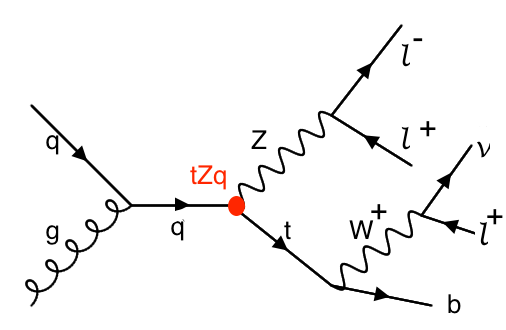
\includegraphics[width=0.35\linewidth]{feynmanST}
%	\includegraphics[width=0.35\linewidth]{feynmanSTtgq}\\
%	\includegraphics[width=0.25\linewidth]{feynmanSTtzq}
%	\includegraphics[width=0.25\linewidth]{feynmanSTtgq2}
%	\caption{\tZ\ Feynman diagrams at leading order. The red vertex indicates the presence of FCNC interactions. The tgq vertices are neglected in the analysis.}
%	\label{fig:feynST}
%\end{figure}
%\begin{figure}[ht]
%	\centering
%	\includegraphics[width=0.35\linewidth]{feynmantttZq}
%	\includegraphics[width=0.25\linewidth]{feynmantttZq2}
%	\caption{\tZq\ Feynman diagram at leading order. The red vertex indicates the presence of FCNC interactions. }
%	\label{fig:feynTT}
%\end{figure}

The signal considers both the single top \FCNC\ (\tZ in the final state) and the top pair \FCNC\ (\tZq in the final state) events. Their final state signatures consist of three leptons, considering electrons or muons in our analysis, and a jet originating from a b quark. For \FCNC\ \tZq, there is an additional up or charm jet. Leptons from tau decays are not vetoed and are also entering the analysis. Therefore, four different lepton channels based on lepton flavour are considered (3e, 2e1$\mu$, 1e2$\mu$, 3$\mu$).  The analysis strategy uses five statistically independent regions to extract limits using a likelihood fit of various observables. Two signal regions, the \tZ\ (\STSR) and \tZq\ (\TTSR) signal region, are constructed using the jet multiplicity,  focussed on each signal signature (see Tab. \ref{tab:Regions}).  In order to constrain the rate of \WZ+jet events as well as that of nonprompt lepton backgrounds three control regions are defined. The \WZ\ control region (\WZCR) focusses on nonprompt leptons originating from \DY\ and simultaneously constrains the \WZ+jets background rate. The nonprompt lepton backgrounds coming from \ttbar, are constrained by two control regions, \TTCR\ and \STCR, one for each signal region (\TTSR\ and \STSR).  In the \STSR\ and \TTSR\, multivariate discriminants based on Boosted Decision Trees (BDT) are used to respectively discriminate \FCNC\ \tZ\ and \FCNC\ \tZq\ from backgrounds. In the \WZCR\ a  discriminating variable between the two backgrounds, \WZ+jets and nonprompt leptons, is used. In \TTCR\ and \STCR\, the dominating process is \ttbar\, and its rate is estimated by subtracting all other background predictions from data. A simultaneous global fit is performed taking into account each region (\STSR, \TTSR, \WZCR, \TTCR\ and \STCR) for the four different leptonic channels. 

\begin{table}[ht]
	\centering
	\caption{The statistically independent regions used in the analysis.}
	\begin{tabular}{c|c|c|c|c|c}
		\hline 
		& \WZ  & \tZ  & \tZq  & \tZ  & \tZq\\ 
		&  control region &  signal region & signal region &  control region & control region\\ 
		& (\WZCR)& (\STSR)  & (\TTSR) & (\STCR) & (\TTCR) \\ 
		\hline 
		Number of jets & $\geqslant 1$, $\leq 3$ & 1 & $\geqslant 2$, $\leq 3$  & 1 & $\geqslant 2$, $\leq 3$\\ 
		\hline 
		Number of b jets & 0 & 1 & $\geqslant 1$  & 1 & $\geqslant 1$ \\ 
		\hline 
		$|M(\PZ_{\mathrm{reco}}) - \mZ|$ & Yes & Yes & Yes & No & No \\
		$< 7.5$ \GeV &  &  &  &  &  \\
		\hline  
	\end{tabular} 
	\label{tab:Regions}
\end{table}


\subsection{WZ control region}
In this region, a fit is performed on the transverse mass of the \PW\ boson, in order to estimate the nonprompt  lepton yield coming from \DY+jets and the \WZ+jets backgrounds. 

A transfer factor has to be used to account for going from a region with 0 b jets to a region with exactly one jet, or at least one jets. For this the probability of tagging at least one jet with the CSVv2 loose working point is used to calculate the expected number of events, Nb, after b tagging: 
\begin{align}
	Nb = \frac{\sum_{events}\text{P(event survives b tag)}}{\text{total nb of events}}
\end{align}
where 
\begin{align}
	\text{P(event survives b tag )} &= 1 - \text{P(event doesn't survive b tag)}\\
	& = 1 - \left(\prod_{b} \text{P(b not tagged)} \prod_{c} \text{P(c not tagged)} \prod_{udsg} \text{P(light not tagged)}\right)\\
	& = 1 - \left(\prod_{b} 0.10 \prod_{c} 0.40 \prod_{udsg} 0.90\right)
\end{align}
with the products going over all b-, c-, and light jets. For this, the jet flavour is taken by means of matching the reconstructed jet to the generated quark based on $\Delta R = \sqrt{\Delta \phi^2 + \Delta \eta^2}$/.  
In order to go to exactly one b jet, this expected number of events is corrected by the fraction of events with exactly  one jet in the \WZCR. The resulting transfer factors are given in Appendix \ref{app:tablestr}. One can see  that the yield of \WZ+jets events in the signal region estimated using the above described transfer factor and the yield calculated with simulated events are in agreement. 

\subsection{\TTCR\ and \STCR}
The \TTCR\ and \STCR have the same selection criteria as \TTSR\ and \STSR\, but are outside the \PZ\ mass window (sidebands): 
\begin{equation}
7.5 \: GeV < |M(Z_{reco}) - M(Z)| < 30 \:GeV. 
\end{equation}
where $M(Z_{reco})$ is the reconstructed mass of the \PZ\ boson in the event, and $M(Z)$ the mass of the \PZ\ boson.
These regions are dominated by \ttbar\ (see Appendix \ref{app:tablestr}) and are used to estimate the nonprompt  leptons coming from \ttbar\ in the \STSR\ and \TTSR. Since there aren't enough events entering these regions, no shapes are used in the fit. The distribution of the mass of the Z boson is flat for \ttbar\ events, as shown in Fig. \ref{fig:3lepcontrolafteratleast1jet3lepzbosonmassallnormalized},  and thus the number of expected events, $Ns$, in the signal regions estimated from the number of expected events, $Nc$, in the control region is obtained as
\begin{equation}
Ns = \frac{15}{60-15} Nc.
\end{equation}
The resulting transfer factors are given in Appendix \ref{app:tablestr}. The expected yield in the signal region estimated from the \TTCR\ (\STCR) is in agreement with the yield calculated from simulated events. 


%\begin{figure}[ht]
%	\centering
%	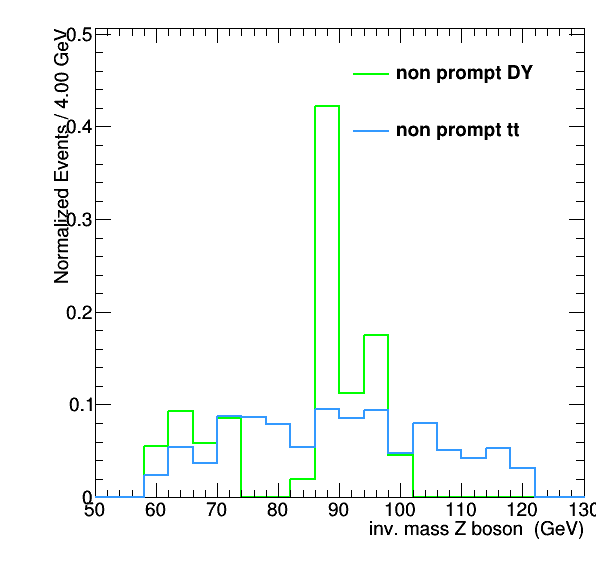
\includegraphics[width=0.47\linewidth]{ZbosonMass/3lepcontrol_afterAtLeast1Jet_3lep__ZbosonMass_all_Normalized}
%	\caption{The normalized distribution for \DY+jets and \ttbar\ events before dividing the events in to regions, after $|M(Z_{\mathrm{reco}}) - M(Z)| < 30$ GeV. All leptonic channels combined.}
%	\label{fig:3lepcontrolafteratleast1jet3lepzbosonmassallnormalized}
%\end{figure}

\subsection{\TTSR\ and \STSR}
The \TTSR\ is defined to target top quark pair FCNC (\tZq), while the \STSR\ focusses on single top quark FCNC (\tZ). They have nonprompt  lepton contributions coming from \DY+jets and \ttbar\ events. In this region, the data driven nonprompt  lepton template is split into two templates based on the presence of the non isolated lepton in the Z boson: 
\begin{itemize}
	\item Non prompt lepton associated with \PW\ boson is assigned to \DY+jets and estimated in the \WZCR.
	\item Non prompt lepton associated with \PZ\ boson is assigned to \ttbar\ and estimated in the \TTCR\ and \STCR.
\end{itemize}
It is shown in Appendix \ref{app:BDTnp}, that these two templates have the same shape within the limited statistics, not assuming any systematic uncertainties. 

\section{Data driven background simulation}
\label{sec:NPL}

The MC samples are used to model the backgrounds as well as for training the boosted decision trees
for signal to background separation. One of the most important background consist of events with nonprompt leptons. These are mostly instrumental background and are therefore very difficult to model. The nonprompt lepton background is estimated from data for both its shape and its normalisation. 

The nonprompt lepton sources are 
\begin{itemize}
	\item hadronic objects wrongly reconstructed as leptons, 
	\item real leptons coming from the semi leptonic decay of a \b\ or \c\ hadron,
	\item real leptons coming from the conversion of photons, 
\end{itemize}
that pass the identification and isolation requirements. The dominant source of these nonprompt leptons depend on the flavour of the lepton and therefore the events with a nonprompt muon are treated differently than those with a nonprompt electron. For muons, the dominant source is the semi leptonic decay of heavy flavour hadrons. For electrons, the dominant sources are hadrons and photon conversions. 

The backgrounds causing nonprompt lepton contributions are mostly Drell--Yan (\DY) and \ttbar\ dilepton processes, and in a smaller amount \WW. All of these backgrounds contain two real leptons and one nonprompt lepton. Due to the fact that the probability for a lepton to be a nonprompt lepton is small, backgrounds containing two or more nonprompt leptons are neglected. The assumption is made that for DY the two leptons compatible with a \PZ\ boson decay are the real leptons, and the additional lepton is coming from a nonprompt lepton source, while for \ttbar\ the nonprompt lepton is associated to the Z boson. 

The nonprompt lepton sample is constructed from data by requiring exactly three leptons, from which two are considered real, isolated leptons and the third is a nonprompt lepton. This nonprompt lepton is created by loosening its identification and inverting its isolation criteria. The full requirements on the (nonprompt) leptons are given in Section \ref{sec:sel}. 
For nonprompt electrons, a large fraction is coming from misidentified photons. These are removed by applying a tighter cut on the $1/E-1/p$ variable, and by limiting the isolation values to be smaller than one (see Table \ref{tab:nonpromptel}). 

The nonprompt leptons samples are defined in a given control region and are used to describe their contribution in the other regions. 
